\section{Detailed Technical Discussion of the Solution}

Technical overview of the solution can be broken down into two main aspects such as features proposed via the new childcare mobile application and high-level proposal for the technical deployment design of the solution.

% \begin{itemize}
%     \item Features proposed via the new childcare mobile application. 
%     \item High-level proposal for the Technical deployment design of the solution.
% \end{itemize}

\subsection{Proposed Features in Mobile Application}

The mobile app for a cenrtalized platform of childcare services offers instant access to vital information, engages parents with notifications, and simplifies center location through geolocation. It allows customization, seamlessly integrates with different existing systems of childcare centers, and will have capability to scale with future updates. \par

\begin{itemize}
    \item \textbf{Mobile-First Accessibility} – A mobile-first approach to childcare services ensures instant access to vital information and services for parents, recognizing their reliance on smartphones for daily tasks.
    \item \textbf{Enhanced Engagement} - The mobile app engages parents with push notifications, updates, and alerts, promoting active participation in childcare.
    \item \textbf{Geolocation Features} - Using mobile device capabilities, the app utilizes geolocation for personalized recommendations, allowing parents to easily find nearby childcare centers and access relevant information, streamlining the search process efficiently.
    \item \textbf{Customizable Preferences} - The mobile app provides personalized experiences, allowing parents to customize preferences and receive tailored recommendations based on their needs. 
    \item \textbf{Seamless Integration} - The app seamlessly integrates with the National Online Portal, providing a unified experience for parents. Data sync ensures consistency in the childcare search process.
    \item \textbf{Scalability and Futureproofing} - The mobile app offers scalability for future enhancements and updates, ensuring its relevance as technology evolves.
\end{itemize}


\subsection{High-Level Deployment Design of the Proposed Solution}

The proposed cross-platform mobile application solution while the backend is proposed to be deployed as microservices on cloud infrastructure, an API gateway for routing, an IAM component for authentication and a scalable database. The proposed design is as follows; 

% \begin{figure*}[htp]
% 	\center
% 	{{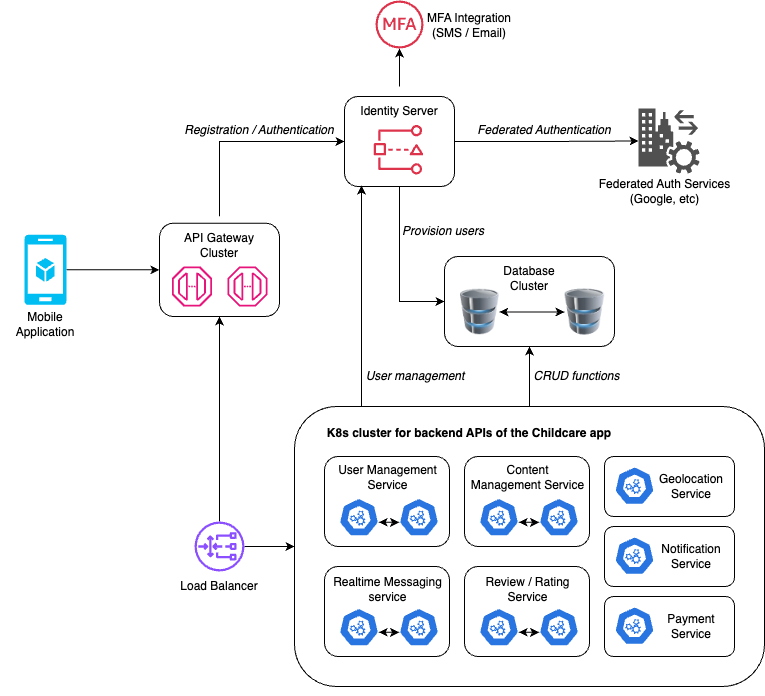
\includegraphics[width=0.55\textwidth,keepaspectratio]{Figures/diagram.png}}}
% 	\caption{Deployment diagram design}%
% 	\label{fig:deploymentdiagram}%
% \end{figure*}

\begin{figure}[htp]
	\center
	{{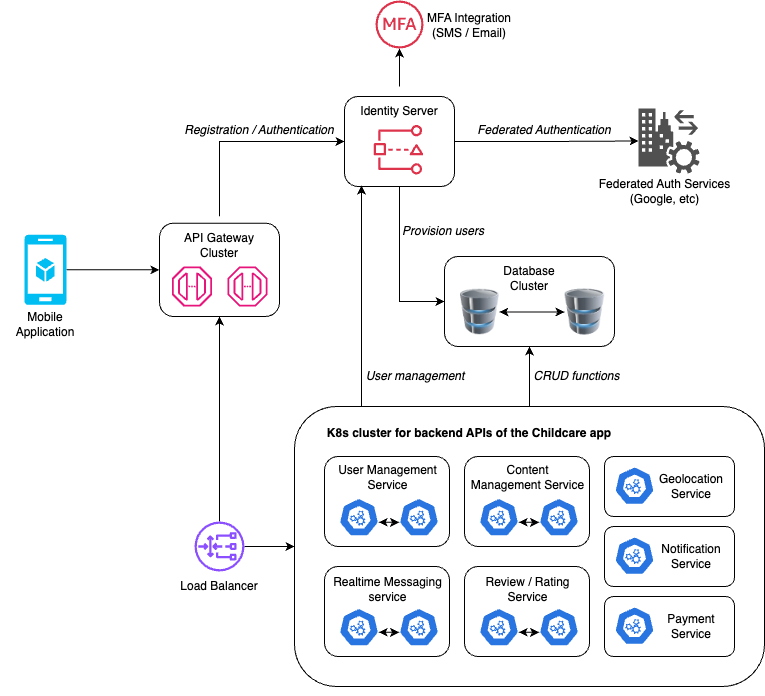
\includegraphics[width=0.9\columnwidth,keepaspectratio]{Figures/diagram.png}}}
	\caption{Deployment design diagram in high-level}%
	\label{fig:deploymentdiagram}%
\end{figure}


\begin{itemize}
    \item \textbf{Mobile Application} – Flutter framework is selected to develop the application due to the cross-platform efficiency, rapid and cost-effective app creation with a single codebase, and dynamic UI components make it a preferred choice for mobile app development. \cite{el2017taxonomy}
    \item \textbf{API Gateway} - MuleSoft has been chosen as the API gateway for its robust features, including centralized management, rate limiting, policy management, and seamless integration with various systems, enabling the development of a scalable and efficient infrastructure. \cite{zylstra2018extended}
    \item \textbf{Load Balancer} - Using a load balancer like Nginx or F5 ensures optimal performance, reliability, scalability, and availability by evenly distributing incoming network traffic, dynamically adjusting server resources, and automatically rerouting traffic away from unhealthy servers. \cite{tudor2009towards}
    \item \textbf{IAM server} - Okta was chosen as a flexible and comprehensive identity management solution that offers customizable policies, automation for streamlined operations, and robust security features including multi-factor authentication. \cite{fang2019okra} 
    \item \textbf{Database Server} - A non-relational database, MongoDB was selected due to it's renowned for supporting complex mobile apps with transactional, search, and analytical features, it excels in managing large volumes of unstructured data with flexibility.
    \item \textbf{Micro-Service Cluster for backend APIs} - Scalability and independent functionalities are enabled through micro-service architecture in this communication platform which helps for flexibility and service uptime maintenance.
\end{itemize}